Post-research we were in a limbo, since the landscape of tooling that can be used for setting up experiments in this field of studies is  quite  vast.
However we decided early in the process that we would mainly work with software simulation, due to the fact that robots have a higher cost and getting the amount of agents that makes these types of studies interesting is somewhat higher than a dozen of robots.

\subsection{Simulation Tools}
Performing simulations is not trivial. Different criteria should be met depending on the accuracy of the simulation that is to be performed.
In particular one should decide what level of abstraction fits the scenario, as 1:1 simulations are significantly harder to model, but might not necessarily add value matching the increased complexity.\\

\textit{This introduces the question, what modelling complexity is sufficient for modelling our problem?}\\

\marginnote{Modelling complexity}
While the real world has three dimensions, we only need a two dimensional model.
The height dimension is not required since we can consider every agent to occupy a space in two dimensional space.\\
Restricting the simulated world to only two axis makes the model a lot simpler to implement.
If this was a simulation for aircrafts the height dimension would make a lot more sense to include,
but in this case all agents lay on the same plane.\\
%Another point is that we need the capability of being able to express physical shapes and collisions between these shapes.\\
%being able to apply kinematic forces to these shapes.

\marginnote{Choice of tools}
Two tools have been considered for implementing the simulated world. One was the GazeboSimulator, which is a widely adopted tool in the robotics community.
Another was doing a simulation using game development tools, in particular Unity3D.

While both tools provide the functionality we need such as physics simulation in 2D/3D  environments, the degree of tools supported out-of-the-box varies.
Gazebo's main function is robotic simulations, and hence it has a lot of useful tools for robotics integrated into it.
Unity3D on the other hand is a general-purpose tool so it requires some tailoring to get the same functionality as Gazebo.

Nevertheless, Unity3D is a strong competitor due to the fact that we have prior experience using this tool, and it has many built in features that handle graphics and physics. 
With little experience, it is easy to go from concept to an actual prototype rapidly.
And last but not least it provides the support of a thriving community of professionals, academics and hobbyists.\\
%aspiring to make the software great.\\
Our solution is built using Unity3D.\\

The choice, albeit it might seem arbitrary, is based on the fact that \textit{Gazebo} has a very steep learning curve.

\begin{figure}
\centering
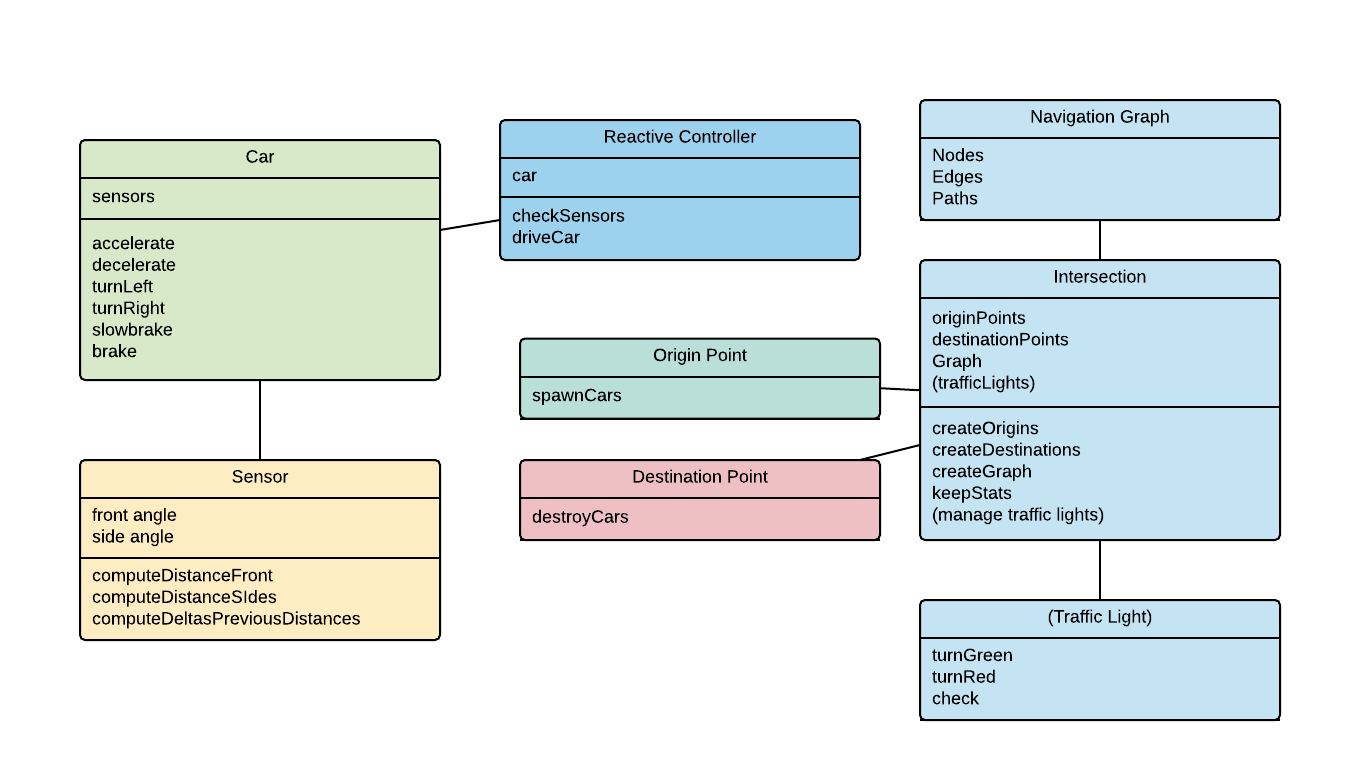
\includegraphics[scale=.6]{img/classdiagram}
\caption{Overview of Unity3D software package}
\label{figure:classdiagram}
\end{figure}

\subsection{Software components}
As we have settled on using Unity3D we work within its boundaries.
It is component driven, meaning every object in the world consists of a collection of components and a transform - the transform is the objects spatial information.
These components can be either colliders, renderers, or custom scripts, and objects can contain other objects as they can be composite.

The implementation was done by splitting the work in three major blocks. One was \textit{the vehicle model}, another was \textit{the intersection model} and the last \textit{the reactive controller} for the car.
An overview of our software package is depicted on figure \ref{figure:classdiagram}.

%\begin{itemize}
%\item Presentation of our model.
%\item Intersection w/wo traffic lights. Cars going straight vs. cars turning.
%\item Car model and sensor modelling (sick vs simplified directional).
%\item Graph for navigation.
%\item Reactive controller.
%\item Special rules (right hand).
%\item Sensor range limitation based on braking distance considerations.
%\item SimScale to RealWorldScale
%\end{itemize}

\subsubsection{The World Model}
As observed in the real world, multiple intersection models exist. Three way and four way intersections are the most common ones.\\
The style can be either with the roundabout approach, which essentially rules out the left turn complication or a traditional four way intersection where going left crosses the opposing traffics lane.

%\textbf{insert simple intersection images - maybe graph images from unity}
\begin{figure}
\centering
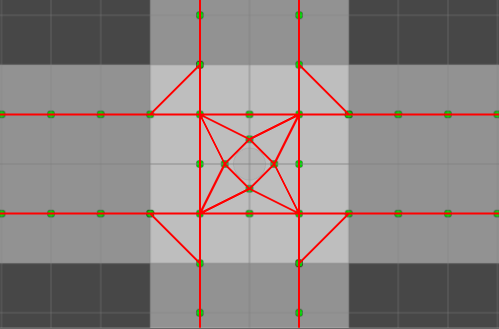
\includegraphics[scale=.4]{img/graph.png}
\caption{Image of the underlying graph representation for a four way intersection.}
\label{figure:graph}
\end{figure}

\begin{figure}
\centering
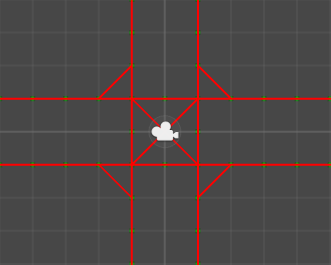
\includegraphics[height=75px]{img/graph-old1.png}
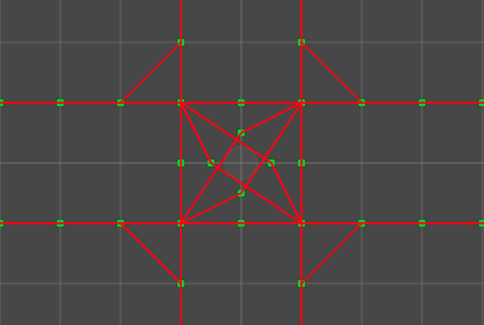
\includegraphics[height=75px]{img/graph-old2.png}
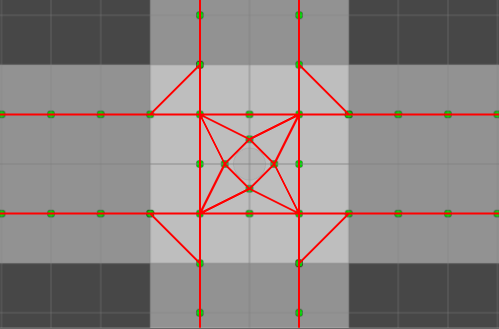
\includegraphics[height=75px]{img/graph-old3.png}
\caption{Image of the previous versions of the underlying navigation graph representation.}
\label{figure:graphs}
\end{figure}

In our model we mainly focus on a single lane 4 way intersection.
We represent these intersection models using an underlying directed graph for navigation.\\
We tried different intersection representations as can be seen on figures \ref{figure:graph} and \ref{figure:graphs}.

A car agent in our environment is seeded with information about its origin and its destination, this is also known as its path.\\
\marginnote{Graph representation}
The origin and destination are vertices in the graph representation.
The paths are made up of a sequence of vertices.
Edges connecting the vertices also contain information about the final destination of that path, in addition to the two vertices it connects.
All vertices figure as control points that a car has to pass through in order to reach a certain destination. \\
After passing each control point, the car controller will check among the edges leaving from that node which one leads to the desired destination.
If the path to the destination is not present in such edges, the default behaviour is to just keep going in the same direction and the next control point is updated.
%Every combination of origin and destination pair has one path.

While this does not provide a lot of flexibility in straying from the path, the simplicity makes the model really easy to implement and adjust.


Once we reached the test phase we also realised that we needed to change measures to real world scale.

\marginnote{World scaling}
We translated our cars to being of a fixed size in meters, and based all the other units according to this value.
This ratio was not arbitrarily chosen, it was based on average values for cars in a certain class.
We looked up car classes on the internet and found something named a compact category.

Compact category covers cars such as Ford Focus, which lengths are between 4.1 and 4.5 meters for hatchbacks and a bit more for sedans, saloons and station wagons.
The car size is of 0.8 units in the simulation environment.

We went with 4.4 meters as being the real world value, and hence got a scaling factor of $5.5$.
Using the scaling factor we also translated the simulated vehicles speeds to km/h, which is quite helpful for the comparisons.

\subsubsection*{The traffic lights}
\marginnote{Traffic light extension}
We introduced traffic lights in an attempt to mimic light regulated intersections.
The lights change at intervals based on data collected doing observations of intersections. 
These values can vary a lot from intersection to intersection - and are highly influenced by traffic flow during the day. 
We performed experiments with different interval windows.

\begin{figure}
\centering
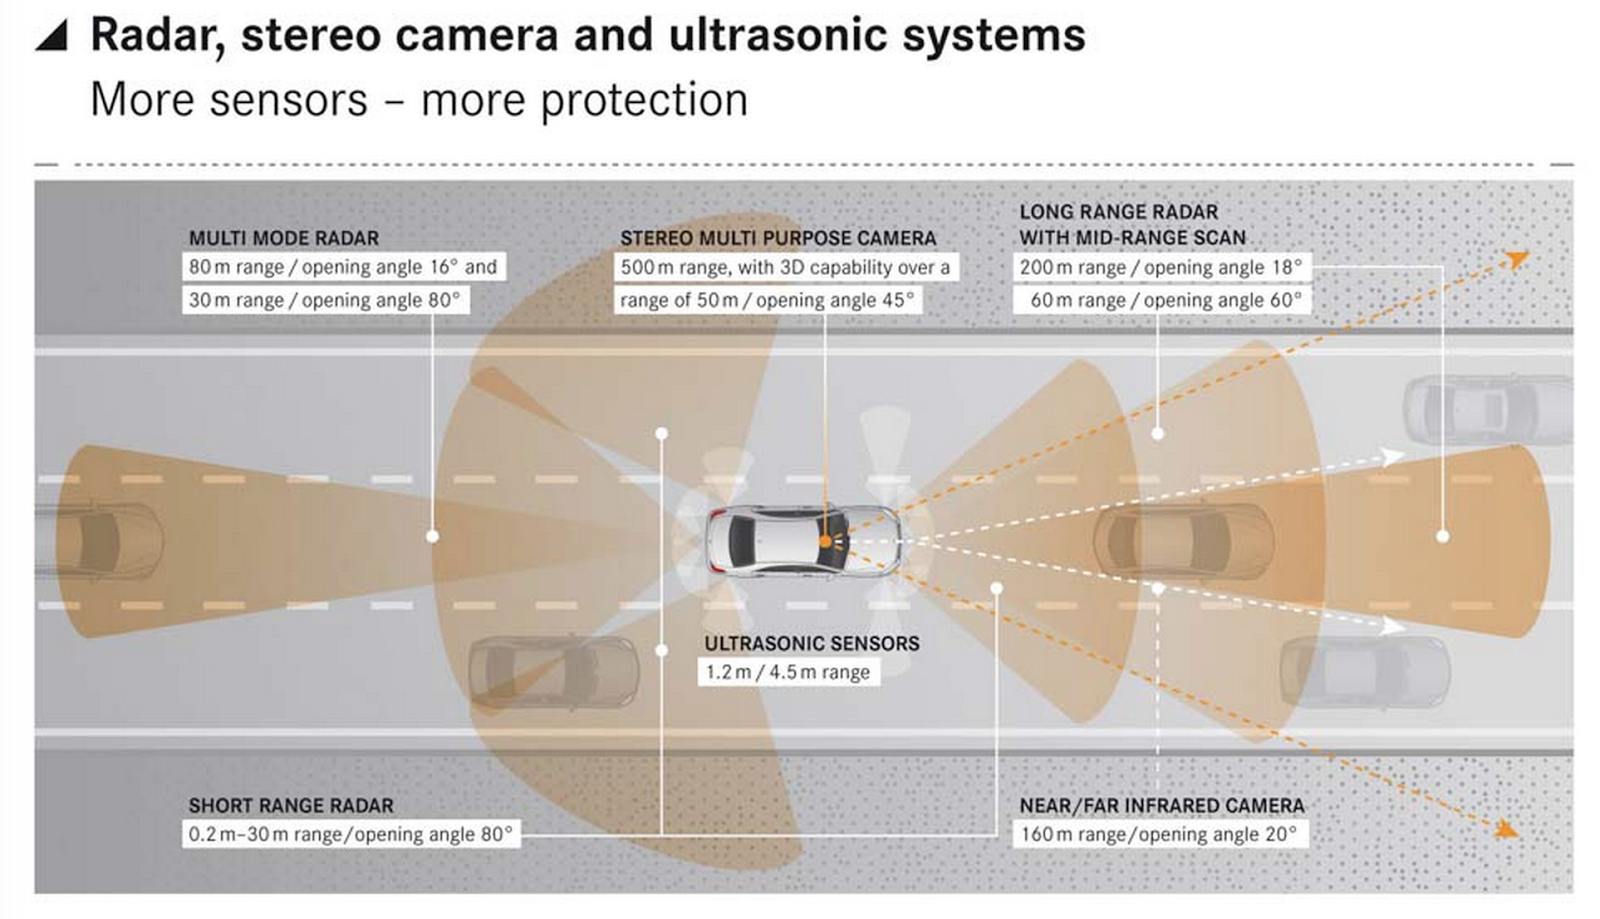
\includegraphics[scale=.2]{img/tesla_sensor}
\caption{Image of the sensors integrated into a car.}
\label{figure:tesla_sens}
\end{figure}

\subsubsection{The Car Model}
The way the car has been modelled is by using an interface which essentially contains actions such as accelerating, decelerating, braking, and turning left or right.
This abstraction simplifies the step of going from a virtual model to a physical one.
The interface provides loose coupling between the controller and the underlying vehicle implementation.
This separation makes it simple to develop multiple types of controllers and vehicles.\\

\begin{figure}
\centering
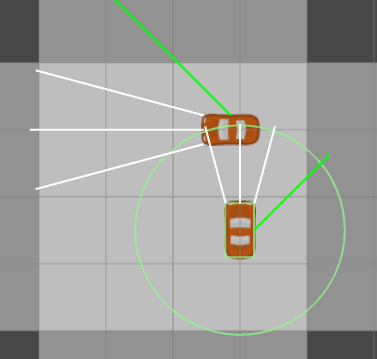
\includegraphics[scale=.5]{img/sensors}
\caption{Image of Unity sensor model.}
\label{figure:unity_sens}
\end{figure}

\subsubsection*{The sensors}
\marginnote{Reference design}
Studying autonomous vehicles, such as the Teslas we realised how much sensing is actually integrated in these marvels.
As seen on figure \ref{figure:tesla_sens}, a lot of sensors exist for achieving autonomous control in vehicles.
The figure is not representative for all autonomous vehicles - but can be seen as a good starting point for understanding the complexity of the vehicles.\\

\marginnote{Hardware investigation}
We focused on mimicking the frontal sensors and the cross-traffic sensors.
We investigated the products of a well-known vendor, SICK, which is used by many different companies within the field.
We mimic 190 degree LMS5xx series for the frontal sensor. This is a sensor which uses lasers. It provides a high degree of precision. It functions in a lot of different conditions and works in the range of 0 to 80 meters\cite{sick}.\\

\marginnote{Sensor implementation}
In our implementation of the sensors, we work with two main angles: $\alpha$ and $\beta$, where $\alpha$  covers the frontal part of the car and $\beta$ the sides.
In figure \ref{figure:unity_sens}, the three white lines represent the $\alpha$ width, which is of $\pi/6$ radiants starting from the centre of the car, and are respectively drawn at [$-\alpha/2, 0, \alpha/2$] angles in relation to the front of the car.\\
Every object detected in this range is considered to be in front of the car.\\

The $\beta$ angle is $\pi$ radiants wide, so everything caught between $\alpha$ and $\beta$ is considered to be to the side of the car.


We also considered that the distance at which to sense other agents should increase with the speed.
This is due to the fact that greater speed results in a longer braking distance, hence the need to react sooner.\\
The sensors' range is represented by the green circle in the figure. \\
The range increases and decreases linearly with the speed of the car, leaving a minimum size that ensures no one enters in too close proximity without notice. 



\subsubsection{The Reactive Controller}
This was developed incrementally. Initial versions were done using only collision avoidance.
The vision was to have multiple different controllers and be able to hot swap these for the simulation.
Later versions also included constructs for priority such as the right hand rule and a finer grained distinction between moving objects and their movement in relation to the agent.\\

\marginnote{Sensor value interpretation}
Due to the simplification of only using one frontal sensor compared to the amount of sensors others might use, we have a finer grained way to interpret the input from this abstraction.
The 180 degree cone is split into zones, which essentially mimics the same division of the frontal senses as seen on figures \ref{figure:tesla_sens} and \ref{figure:unity_sens}.
We took the abstraction further and limited the range of detection based on velocity of the vehicle. The faster it goes the farther it looks ahead.
This reduces the risk of vehicles being overly cautious and stopping in intersections with lots of slow moving vehicles, especially if it is still possible to pass through.
Additionally the braking distance is not as big at lower velocities - which makes this approach reasonable.\\

\marginnote{Collision avoidance}
The controller has been reiterated multiple times: initially it was only doing collision avoidance.
This was achieved by acting directly on the frontal sensor values.\\
The earliest versions only had one threshold. If anything was closer than the given threshold the car would not move.
While this avoids colliding with anything in front, it does not handle cross-traffic well.\\
We did another version which trails behind the car in front.
This is done using the delta distance rather than raw distance.
For delta distance it is meant the difference between the distance measured at a given time $t$, and the same distance measured at $t-1$. 
If two vehicles move at the same speed, one in front of the other, their distance is constant and the delta stays zero.
If the gap closes, the delta gains a negative value and the controller can react by braking. 
